\hypertarget{a00014}{
\section{eqOsg::Pipe Class Reference}
\label{a00014}\index{eqOsg::Pipe@{eqOsg::Pipe}}
}
The \hyperlink{a00014}{Pipe} holds the viewer and the frame data.  


{\tt \#include $<$Pipe.h$>$}

Inherited by \hyperlink{a00006}{crf::crfPipe}.

Collaboration diagram for eqOsg::Pipe:\nopagebreak
\begin{figure}[H]
\begin{center}
\leavevmode
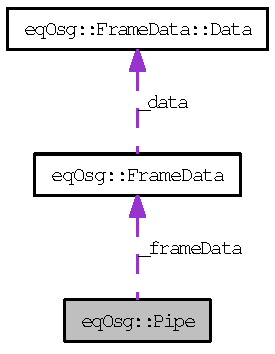
\includegraphics[width=168pt]{a00101}
\end{center}
\end{figure}
\subsection*{Public Member Functions}
\begin{CompactItemize}
\item 
\hyperlink{a00014_70ba41100439b9cd50a7aeea8060d5ac}{Pipe} (eq::Node $\ast$parent)
\item 
const \hyperlink{a00010}{FrameData} \& \hyperlink{a00014_b0c77c44b8b387666ef45b76bc8d2284}{getFrameData} () const 
\begin{CompactList}\small\item\em Returns the pipe's \hyperlink{a00010}{FrameData} object. \item\end{CompactList}\item 
osg::ref\_\-ptr$<$ \hyperlink{a00009}{eqOsg::EqViewer} $>$ \hyperlink{a00014_e0cf2ae4fae2e59cbb65374084c8b563}{getViewer} () const 
\begin{CompactList}\small\item\em Returns the pipe's \hyperlink{a00009}{EqViewer}. \item\end{CompactList}\end{CompactItemize}
\subsection*{Protected Member Functions}
\begin{CompactItemize}
\item 
virtual bool \hyperlink{a00014_d23bd6f7bb0f59f94fc0e279dbbb9d9a}{configInit} (const uint32\_\-t initID)
\begin{CompactList}\small\item\em Registers the frame data, so it can be synced with the server later. \item\end{CompactList}\item 
virtual bool \hyperlink{a00014_2cb47387a7be185b1dc6d097dc4da38e}{configExit} ()
\begin{CompactList}\small\item\em Deregisters the frame data. \item\end{CompactList}\item 
virtual void \hyperlink{a00014_6be431b1b9fe04da31596ea8b870dfde}{frameStart} (const uint32\_\-t frameID, const uint32\_\-t frameNumber)
\begin{CompactList}\small\item\em Syncs the frame data with the server and calls updateSceneGraph(). \item\end{CompactList}\item 
virtual void \hyperlink{a00014_bb1e29569fab6e079fc1fcb286af4f40}{createSceneGraph} (std::string modelFileName)
\begin{CompactList}\small\item\em Creates a scene graph with a model by filename. \item\end{CompactList}\item 
virtual osg::ref\_\-ptr$<$ osg::Node $>$ \hyperlink{a00014_b357cd9e8e214f839388de82e14333a1}{correctCoordsys} (osg::ref\_\-ptr$<$ osg::Node $>$ nodeToRotate)
\begin{CompactList}\small\item\em Corrects the coordination system from osg to eq. \item\end{CompactList}\item 
osg::ref\_\-ptr$<$ osg::Node $>$ \hyperlink{a00014_7f42242765d3cb5b0132bfc5c8ed7142}{correctCoordsys} (osg::ref\_\-ptr$<$ osg::Node $>$ nodeToTransform, osg::Matrix matrix)
\begin{CompactList}\small\item\em Transform a desired node around a passed matrix. \item\end{CompactList}\end{CompactItemize}
\subsection*{Protected Attributes}
\begin{CompactItemize}
\item 
\hypertarget{a00014_b4f8193b938ef155c87df88e084e42fc}{
\hyperlink{a00010}{FrameData} \hyperlink{a00014_b4f8193b938ef155c87df88e084e42fc}{\_\-frameData}}
\label{a00014_b4f8193b938ef155c87df88e084e42fc}

\begin{CompactList}\small\item\em The \hyperlink{a00010}{FrameData} object. \item\end{CompactList}\item 
\hypertarget{a00014_e36ebe17666eeda7d5293077a69ba6ad}{
osg::ref\_\-ptr$<$ \hyperlink{a00009}{eqOsg::EqViewer} $>$ \hyperlink{a00014_e36ebe17666eeda7d5293077a69ba6ad}{\_\-viewer}}
\label{a00014_e36ebe17666eeda7d5293077a69ba6ad}

\begin{CompactList}\small\item\em The pipe's \hyperlink{a00009}{EqViewer}. \item\end{CompactList}\item 
\hypertarget{a00014_c58577ad857d962e3f4da22492911631}{
bool \hyperlink{a00014_c58577ad857d962e3f4da22492911631}{\_\-sceneGraphCreated}}
\label{a00014_c58577ad857d962e3f4da22492911631}

\begin{CompactList}\small\item\em Set to true if the scene graph has been created and added to the viewer. \item\end{CompactList}\item 
\hypertarget{a00014_ac2035c8102ec6a66160453963b1d9b4}{
bool \hyperlink{a00014_ac2035c8102ec6a66160453963b1d9b4}{\_\-usesModel}}
\label{a00014_ac2035c8102ec6a66160453963b1d9b4}

\begin{CompactList}\small\item\em Set to true if a simple model shoudl be load. \item\end{CompactList}\item 
\hypertarget{a00014_4cc32263a7c4cb68639f65bc7a18ca49}{
std::string \hyperlink{a00014_4cc32263a7c4cb68639f65bc7a18ca49}{\_\-modelFile}}
\label{a00014_4cc32263a7c4cb68639f65bc7a18ca49}

\begin{CompactList}\small\item\em The filename of the to-load model. \item\end{CompactList}\end{CompactItemize}


\subsection{Detailed Description}
The \hyperlink{a00014}{Pipe} holds the viewer and the frame data. 

Each frame, it updates the scene graph of the viewer with the new data of the frame data. The frame data is synced with the server. \begin{Desc}
\item[See also:]eq::Pipe \end{Desc}


\subsection{Constructor \& Destructor Documentation}
\hypertarget{a00014_70ba41100439b9cd50a7aeea8060d5ac}{
\index{eqOsg::Pipe@{eqOsg::Pipe}!Pipe@{Pipe}}
\index{Pipe@{Pipe}!eqOsg::Pipe@{eqOsg::Pipe}}
\subsubsection[{Pipe}]{\setlength{\rightskip}{0pt plus 5cm}Pipe::Pipe (eq::Node $\ast$ {\em parent})}}
\label{a00014_70ba41100439b9cd50a7aeea8060d5ac}


\begin{Desc}
\item[See also:]eq::Pipe::Pipe \end{Desc}


\subsection{Member Function Documentation}
\hypertarget{a00014_2cb47387a7be185b1dc6d097dc4da38e}{
\index{eqOsg::Pipe@{eqOsg::Pipe}!configExit@{configExit}}
\index{configExit@{configExit}!eqOsg::Pipe@{eqOsg::Pipe}}
\subsubsection[{configExit}]{\setlength{\rightskip}{0pt plus 5cm}bool Pipe::configExit ()\hspace{0.3cm}{\tt  \mbox{[}protected, virtual\mbox{]}}}}
\label{a00014_2cb47387a7be185b1dc6d097dc4da38e}


Deregisters the frame data. 

\begin{Desc}
\item[Returns:]True if everything worked fine. \end{Desc}


Reimplemented in \hyperlink{a00006_3f48f5f5a8a455342b111f26ca1402db}{crf::crfPipe}.\hypertarget{a00014_d23bd6f7bb0f59f94fc0e279dbbb9d9a}{
\index{eqOsg::Pipe@{eqOsg::Pipe}!configInit@{configInit}}
\index{configInit@{configInit}!eqOsg::Pipe@{eqOsg::Pipe}}
\subsubsection[{configInit}]{\setlength{\rightskip}{0pt plus 5cm}bool Pipe::configInit (const uint32\_\-t {\em initID})\hspace{0.3cm}{\tt  \mbox{[}protected, virtual\mbox{]}}}}
\label{a00014_d23bd6f7bb0f59f94fc0e279dbbb9d9a}


Registers the frame data, so it can be synced with the server later. 

\begin{Desc}
\item[Parameters:]
\begin{description}
\item[{\em initID}]The Equalizer initID. \end{description}
\end{Desc}
\begin{Desc}
\item[Returns:]True if everything worked fine. \end{Desc}


Reimplemented in \hyperlink{a00006_fcf11863d5370a815bd7e1216cc0f2e6}{crf::crfPipe}.\hypertarget{a00014_7f42242765d3cb5b0132bfc5c8ed7142}{
\index{eqOsg::Pipe@{eqOsg::Pipe}!correctCoordsys@{correctCoordsys}}
\index{correctCoordsys@{correctCoordsys}!eqOsg::Pipe@{eqOsg::Pipe}}
\subsubsection[{correctCoordsys}]{\setlength{\rightskip}{0pt plus 5cm}osg::ref\_\-ptr$<$ osg::Node $>$ Pipe::correctCoordsys (osg::ref\_\-ptr$<$ osg::Node $>$ {\em nodeToTransform}, \/  osg::Matrix {\em matrix})\hspace{0.3cm}{\tt  \mbox{[}protected\mbox{]}}}}
\label{a00014_7f42242765d3cb5b0132bfc5c8ed7142}


Transform a desired node around a passed matrix. 

\begin{Desc}
\item[Parameters:]
\begin{description}
\item[{\em nodeToTransform}]The node, which should be transformed. \item[{\em matrix}]The transformation matrix. \end{description}
\end{Desc}
\begin{Desc}
\item[Returns:]The transformed node. \end{Desc}
\hypertarget{a00014_b357cd9e8e214f839388de82e14333a1}{
\index{eqOsg::Pipe@{eqOsg::Pipe}!correctCoordsys@{correctCoordsys}}
\index{correctCoordsys@{correctCoordsys}!eqOsg::Pipe@{eqOsg::Pipe}}
\subsubsection[{correctCoordsys}]{\setlength{\rightskip}{0pt plus 5cm}osg::ref\_\-ptr$<$ osg::Node $>$ Pipe::correctCoordsys (osg::ref\_\-ptr$<$ osg::Node $>$ {\em nodeToRotate})\hspace{0.3cm}{\tt  \mbox{[}protected, virtual\mbox{]}}}}
\label{a00014_b357cd9e8e214f839388de82e14333a1}


Corrects the coordination system from osg to eq. 

Rotates the whole scene 90� around the X-axis and 180 around Y to fit the commonly used Equalizer schema. \begin{Desc}
\item[Parameters:]
\begin{description}
\item[{\em nodeToRotate}]The node, which should be rotated \end{description}
\end{Desc}
\begin{Desc}
\item[Returns:]The rotated node \end{Desc}
\hypertarget{a00014_bb1e29569fab6e079fc1fcb286af4f40}{
\index{eqOsg::Pipe@{eqOsg::Pipe}!createSceneGraph@{createSceneGraph}}
\index{createSceneGraph@{createSceneGraph}!eqOsg::Pipe@{eqOsg::Pipe}}
\subsubsection[{createSceneGraph}]{\setlength{\rightskip}{0pt plus 5cm}void Pipe::createSceneGraph (std::string {\em modelFileName})\hspace{0.3cm}{\tt  \mbox{[}protected, virtual\mbox{]}}}}
\label{a00014_bb1e29569fab6e079fc1fcb286af4f40}


Creates a scene graph with a model by filename. 

\begin{Desc}
\item[Parameters:]
\begin{description}
\item[{\em modelFileName}]The filename of the model. \end{description}
\end{Desc}
\hypertarget{a00014_6be431b1b9fe04da31596ea8b870dfde}{
\index{eqOsg::Pipe@{eqOsg::Pipe}!frameStart@{frameStart}}
\index{frameStart@{frameStart}!eqOsg::Pipe@{eqOsg::Pipe}}
\subsubsection[{frameStart}]{\setlength{\rightskip}{0pt plus 5cm}void Pipe::frameStart (const uint32\_\-t {\em frameID}, \/  const uint32\_\-t {\em frameNumber})\hspace{0.3cm}{\tt  \mbox{[}protected, virtual\mbox{]}}}}
\label{a00014_6be431b1b9fe04da31596ea8b870dfde}


Syncs the frame data with the server and calls updateSceneGraph(). 

\begin{Desc}
\item[See also:]eq::Pipe::frameStart \end{Desc}


Reimplemented in \hyperlink{a00006_2e551fe08841da2b7a1def541656d48c}{crf::crfPipe}.\hypertarget{a00014_b0c77c44b8b387666ef45b76bc8d2284}{
\index{eqOsg::Pipe@{eqOsg::Pipe}!getFrameData@{getFrameData}}
\index{getFrameData@{getFrameData}!eqOsg::Pipe@{eqOsg::Pipe}}
\subsubsection[{getFrameData}]{\setlength{\rightskip}{0pt plus 5cm}const {\bf FrameData} \& Pipe::getFrameData () const}}
\label{a00014_b0c77c44b8b387666ef45b76bc8d2284}


Returns the pipe's \hyperlink{a00010}{FrameData} object. 

\begin{Desc}
\item[Returns:]The \hyperlink{a00010}{FrameData} of this pipe. \end{Desc}
\hypertarget{a00014_e0cf2ae4fae2e59cbb65374084c8b563}{
\index{eqOsg::Pipe@{eqOsg::Pipe}!getViewer@{getViewer}}
\index{getViewer@{getViewer}!eqOsg::Pipe@{eqOsg::Pipe}}
\subsubsection[{getViewer}]{\setlength{\rightskip}{0pt plus 5cm}osg::ref\_\-ptr$<$ {\bf EqViewer} $>$ Pipe::getViewer () const}}
\label{a00014_e0cf2ae4fae2e59cbb65374084c8b563}


Returns the pipe's \hyperlink{a00009}{EqViewer}. 

\begin{Desc}
\item[Returns:]The Eqviewer of this pipe. \end{Desc}


The documentation for this class was generated from the following files:\begin{CompactItemize}
\item 
E:/schule/Thesis/Repo/trunk/crf/src/Pipe.h\item 
E:/schule/Thesis/Repo/trunk/crf/src/Pipe.cpp\end{CompactItemize}
